\documentclass[letterpaper,openany,twoside,twocolumn]{book}

\newcommand{\PATH}{../../../}

\usepackage[justified]{\PATH dndtemplate/dnd}

\usepackage{\PATH regions/stylesheets/monster_book_commands}
\usepackage{\PATH regions/stylesheets/regions_stylesheet}
\usepackage{\PATH regions/stylesheets/dungeon_stylesheet}
\usepackage{\PATH regions/stylesheets/monster_stylesheet}
\usepackage{\PATH regions/stylesheets/shadowfy}

\usepackage[english]{babel}
\usepackage[utf8]{inputenc}

%\newcommand{\entryfont}{\DndFontStatBlockBody} & uses the default font provided by the LaTeX DnD-Template
\newfontfamily\entryfont{Kalam}[Path=\PATH template/fonts/,Extension=.ttf,UprightFont=Kalam-Regular,BoldFont=Kalam-Bold] % requires XeLaTeX or LuaTeX
\newfontfamily\titlefont{Modesto Bold(2)}[Path=\PATH template/fonts/,Extension=.otf,UprightFont=Modesto Bold(2),BoldFont=Modesto Bold(2)] % requires XeLaTeX or LuaTeX

\AtBeginDocument{\addtocontents{toc}{\protect\thispagestyle{empty}}}

\begin{document}
	% Titlepage	
	\monstersTitlePage{Serpent's Embrace}{images/titlepage_Serpent's_Embrace.jpg}{0.5cm}{0cm}{height=\paperheight}{https://www.artstation.com/artwork/QrEPaE}{Desert Serpent}{Jannis Mayr}{A collection of homebrew monsters found in the Serpent's Embrace Desert}
	
	\tableofcontents
	
	\mainmatter
	
	\graphicspath{{./images},{./monsters/Ebony_Scarab/images}}

\MonsterSheetGeometry

% --------------------------------------------------------------------------------------------------- %
% ################################################################################################### %
% #-#-#-#-#-#-#-#-#-#-#-#-#-#-# Monster-Sheet with two Smaller Pictures #-#-#-#-#-#-#-#-#-#-#-#-#-#-# %
% ################################################################################################### %
% --------------------------------------------------------------------------------------------------- %

\chapter*{Ebony Scarab}
\stepcounter{chapter}
\addcontentsline{toc}{chapter}{\protect\numberline{\thechapter}Ebony Scarab}

\entryfont \noindent \DndDropCapLine{H}ailing from the depths of arid deserts and sun-scorched wastelands, the Ebony Scarab is a marvel of natural engineering. Its chitinous exoskeleton shimmers with a rich hue of black or dark blue, akin to the darkest nights. Yet, this profound darkness is not devoid of life, for intricate golden accents dance across its carapace, capturing the very essence of stardust. These gilded highlights mark its eyes, mandibles, and the fine lines that trace patterns along its armor, a testament to the creature's innate mystique.\\

The Ebony Scarab stands at a formidable 4 to 5 feet in height, its presence radiating an eerie intelligence from its multifaceted, gleaming eyes. Its antennae, in a constant state of delicate twitching, seem to tap into the very vibrations of the earth. As it moves, the sand and soil beneath its feet seem to part willingly, acknowledging the ancient power it wields.\\

This creature's demeanor is a fascinating blend of the graceful and the fearsome. It carries itself with an almost regal bearing, its plated limbs moving with a fluid grace that belies its size. Yet, its mandibles, powerful enough to crush stone and bone alike, provide a constant reminder of its primal nature. When it locks eyes with its prey, an unsettling aura envelops its gaze, capable of instilling terror in even the most resolute souls.\\

Amidst the barren landscapes it calls home, the Ebony Scarab is a master of camouflage. Its exoskeleton, versatile as an artist's palette, can morph to match its surroundings—vanishing into shadows, or blending seamlessly with sand and rock. This natural gift, combined with its keen senses, makes it a predator that strikes from hidden lairs and buried tunnels.

\MonsterGraphicAndShortInfo{shortinfo}% shortinfo or none for no Short-Info Box
{%
	{-8cm}% Shift Horizontal Short Info Box
	{5.5cm}% Shift Vertical Short Info Box
	{25}% Rotation Angle Short Info Box
	{4.5cm}% Width of Short-Info Box
	{6}% Number of Lines in Textbox (might be adjusted after 1 compile) 
	{%
		A meeting with the Ebony Scarab, whether beneath the sun's unforgiving gaze or the starlit canopy of night, is an encounter with the mysteries of the desert - majestic, deadly, and filled with the allure of the unknown.%
	}%
}%
{-0.25cm}% Shift Horizontal Monster Graphic
{0.05cm}% Shift Vertical Monster Graphic
{, anchor=south west}% Further Picture Placement Options
{(current page.south west)}% Anchor-Point on Page
{height=300pt, width=1.5\textwidth}% Dimension of Graphic
{Ebony_Scarab.png}%
\addImageDBEntry{BlankMonster1}% Handle for the page reference, must be individual for each image
	{Page \thepage}% Display for page numbering. No need for change
	{Monster Art}% more accurate Identifer (BAckground Art, Variant Art, etc.)
	{https://www.deviantart.com/yirikus/art/Ancient-Beetle-Guardian-892850845}% URL to picture or graphic
	{Ancient Beetle Guardian}% Name of Art
	{Yirikus}% Artist

\vfill\eject % cammand to break to next column

\vspace*{-5cm}
\begin{center}\begin{tikzpicture}
	\node[inner sep=0pt, outer sep=0pt, rotate=60] {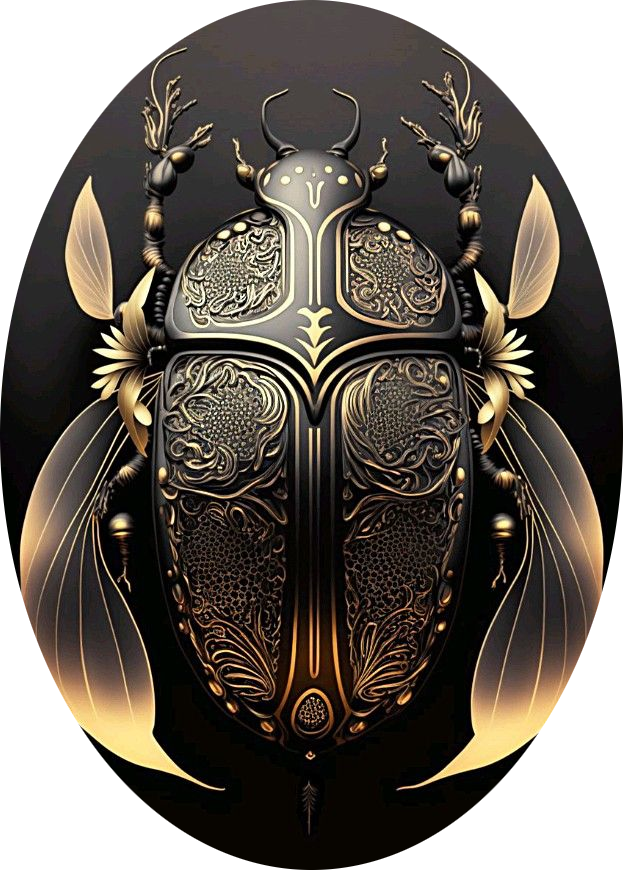
\includegraphics[height=\columnwidth-30pt, keepaspectratio]{Ebony_Scarab_Token.png}};
\end{tikzpicture}\end{center}
\vspace*{-2cm}
% Monster stat block
\begin{DndMonster}[width=0.5\textwidth]{Ebony Scarab}
    \DndMonsterType{Medium Monstrosity, neutral}

    % If you want to use commas in the key values, enclose the values in braces.
    \DndMonsterBasics[
        armor-class = {15 (Natural Armor)},
        hit-points  = {\DndDice{6d8 + 18}},
        speed       = {30 ft., burrow 20 ft.},
    ]
    
	\renewcommand{\AbilityScoreSpacer}{~}
    \DndMonsterAbilityScores[
		str = 16,
		dex = 14,
		con = 16,
		int = 6,
		wis = 12,
		cha = 7,
    ]

    \DndMonsterDetails[
        %saving-throws = {Str +0, Dex +0, Con +0, Int +0, Wis +0, Cha +0},
        skills = {Perception +3, Stealth +4},
        %damage-vulnerabilities = {cold},
        %damage-resistances = {bludgeoning, piercing, and slashing from nonmagical attacks},
        damage-immunities = {poison},
        senses = {Darkvision 60 ft., Tremorsense 30 ft., Passive Perception 13},
        condition-immunities = {poisoned},
        %languages = {-},
        challenge = 2,
    ]
    
    \DndMonsterAction{Chitinous Armor}
    The Ebony Scarab has a +3 bonus to its Armor Class due to its tough exoskeleton.
	
	\DndMonsterSection{Actions}	
	\DndMonsterAttack[
      name=Crushing Mandibles,
      distance=melee, % valid options are in the set {both,melee,ranged},
      %type=weapon, %valid options are in the set {weapon,spell}
      mod=+5,
      reach=5,
      %range=20/60,
      targets=one target,
      dmg=\DndDice{1d10 + 3},
      dmg-type=slashing,
      %plus-dmg=,
      %plus-dmg-type=,
      %or-dmg=,
      %or-dmg-when=,
      %extra=,
    ]
    
	\DndMonsterAction{Eerie Gaze}
	The Ebony Scarab targets one creature it can see within 30 feet of it. The target must succeed on a DC 13 Wisdom saving throw or be frightened until the end of its next turn.
	
	\DndMonsterAttack[
      name=Infectious Sting,
      distance=melee, % valid options are in the set {both,melee,ranged},
      %type=weapon, %valid options are in the set {weapon,spell}
      mod=+2,
      reach=5,
      %range=20/60,
      targets=one target,
      %dmg=,
      %dmg-type=slashing,
      %plus-dmg=,
      %plus-dmg-type=,
      %or-dmg=,
      %or-dmg-when=,
      extra={The target must make a DC 12 Constitution saving throw or be paralyzed for 1 minute. The target can repeat the saving throw at the end of each of its turns, ending the effect on a success},
    ]
	
	\DndMonsterSection{Reactions}
	\DndMonsterAction{Chromatic Shift}
	When a creature targets the Ebony Scarab with an attack, the scarab can use its reaction to shift its color, imposing disadvantage on the attack roll.
	
\end{DndMonster}
	\graphicspath{{./images},{./monsters/Giant_Sandweaver/images}}

\MonsterSheetGeometry

\chapter*{Giant Sandweaver}
\stepcounter{chapter}
\addcontentsline{toc}{chapter}{\protect\numberline{\thechapter}Giant Sandweaver}
\vspace*{-2.4\fontdimen6\font}

\entryfont \noindent \DndDropCapLine{N}ative to sandy deserts and shrugged canyons, the Giant Sandweaver is a horrendous sight to encounter. Different to common spiders these monsters do not spin large intricate webs, but instead cover large areas of their territory with a thick weave of silk to act as an alarm system for intruders. Furthermore, Giant Sandweaver live in large families, similar to hives, which form around a matriarch - a so-called Sandwidow.\\
\textbf{Appearance.} Giant Sandweavers are large serpents that can reach lengths of up to 12 feet and have 6-8 spider-like legs. Individual specimens, especially Sandwidows, are said to have been up to 15 feet in length. The body itself is covered by hard plates, giving a very good resistance to any attack. Closer to the head these bodyplates form massive spikes. While the Giant Sandweaver is buried in the sand these spikes might be mistaken for stones or obelisk by unaware travellers.\\
\textbf{Ritual Abomination.} The first Giant Sandweavers were created in dark rituals by the lizardfolk tribe Yuan-Shu during the war with the Yuan-Ti. These were released in crucial positions, most commonly canyons, to hinder the advances of the opponent's troops and attack any snakefolk that trespasses the terrain. The Yuan-Shu relished in the idea of turning snakes into spider-like monsters that preyed upon the snake worshipping Yuan-Ti, a metaphor of the lizardfolk's superiority.\\
During combat the Giant Sandweaver tries to catch or incapacitate its opponents within its webbing. Already caught opponents are not the preferred target if other non-incapacitated opponents are around.\\
\textbf{Monstrous Mounts.} Over the centuries, Yuan-Ti were able to tame some Giant Seandweavers just enough to serve as mounts in combat. However, Giant Sandweaver are notoriously treacherous creatures and their alliance usually lies with whoever feeds them.\\
- M4RZ.\\

\MonsterGraphicAndShortInfo{shortinfo}% shortinfo or none for no Short-Info Box
{%
	{1.15cm}% Shift Horizontal Short Info Box
	{5.65cm}% Shift Vertical Short Info Box
	{-12}% Rotation Angle Short Info Box
	{3.7781cm}% Width of Short-Info Box
	{8}% Number of Lines in Textbox (might be adjusted after 1 compile) 
	{%
		First created by the Yuan-Shu to gain an advantage in combat and war, these spider-like serpents roam through the vast deserts and deep canyons.\\These monsters are formidable foes and it is ill-advised to mess with their hive. %
	}%
}%
{0.75cm}% Shift Horizontal Monster Grpahic
{0.05cm}% Shift Vertical Monster Grpahic
{, anchor=south west}% Further Picture Placement Options
{(current page.south west)}% Anchor-Point on Page
{height=325pt}% Dimension of Graphic
{Giant_Sandweaver.png}%
\addImageDBEntry{Sandweaver1}{Page \thepage}{Art}{https://static.wikia.nocookie.net/alchemystars/images/7/7c/Mara_Sol.png/revision/latest/scale-to-width-down/1000?cb=20210814053823}{Mara Sol}{Alchemy Stars}%

\vfill\eject

\MonsterVariant{-1em}%
	{Giant_Sandweaver_variant.png}%
	{-1cm} % distance offset from image to Variant Box
	{Sandwidow}%
	{%
		The matriarch of a Giant Sandweaver family has more similarities to an actual snake and its legs are covered in hair, that can detect pressure differences and air movement in the Sandwidow's surroundings.
		\DndMonsterAction{Hit Points} {\footnotesize \DndDice{15d12 + 66}}
		\DndMonsterAction{Pit organs}
		{\footnotesize The Sandwidow has blindsight in a 50 ft. radius, on creatures whose body temperature is more than half than the temperature of its surroundings.}
		\DndMonsterAction{Trichobothria}
		{\footnotesize The Sandwidow can detect movement within a 100ft. radius.}
		\DndMonsterAction{Spit Venom (Recharge 5-6)}
		{\footnotesize The Sandwidow spits venom in a 40 foot line that is 5 feet wide. Each creature in that line must make a DC 18 Constitution saving throw, taking \DndDice{6d8 + 6} poison damage on a failed save, or half as much on a successful one.}
	}%
	\addImageDBEntry{Sandweaver2}{Page \thepage}{Variant Art}{https://www.artstation.com/artwork/4wXGq}{Tarantuviper}{Dave Melvin}%
\vspace*{-1.5em}
% Monster stat block
\begin{DndMonster}[width=0.5\textwidth]{Giant Sandweaver}
    \DndMonsterType{Huge monstrosity, unaligned}

    % If you want to use commas in the key values, enclose the values in braces.
    \DndMonsterBasics[
        armor-class = {18 (natural armor)},
        hit-points  = {\DndDice{8d12 + 42}},
        speed       = {30 ft., climb 25 ft., dig/tunneling 25 ft.},
      ]

    \DndMonsterAbilityScores[
        str = 19,
        dex = 15,
        con = 21,
        int = 6,
        wis = 9,
        cha = 5,
      ]

    \DndMonsterDetails[
        %saving-throws = {Str +0, Dex +0, Con +0, Int +0, Wis +0, Cha +0},
        %skills = {Acrobatics +0, Animal Handling +0, Arcana +0, Athletics +0, Deception +0, History +0, Insight +0, Intimidation +0, Investigation +0, Medicine +0, Nature +0, Perception +0, Performance +0, Persuasion +0, Religion +0, Sleight of Hand +0, Stealth +0, Survival +0},
        %damage-vulnerabilities = {cold},
        damage-resistances = {bludgeoning, piercing, and slashing from nonmagical attacks (not Sandwidow), poison},
        %damage-immunities = {cold},
        senses = {passive Perception 14},
        condition-immunities = {frightened, poisoned, prone},
        languages = {Primordial},
        challenge = 9,
      ]
      
    \DndMonsterAction{Spider Climb}
    The Giant Sandweaver can climb difficult surfaces, including upside down ceilings, without the need of an ability check.
      
    \DndMonsterAction{Web Sense}
    While in contact with a web, the Giant Sandweaver knows the exact location of any other creature in contact with the same web.
      
    \DndMonsterSection{Actions}
	\DndMonsterAction{Multiattack}
	The Giant Sandweaver can attack twice each turn.   
    
    \DndMonsterAttack[
      name=Poisonous Bite,
      distance=melee, % valid options are in the set {both,melee,ranged},
      %type=weapon, %valid options are in the set {weapon,spell}
      mod=+7,
      reach=5,
      %range=20/60,
      targets=one target,
      dmg={\DndDice{2d6 + 1}},
      dmg-type=piercing,
      %plus-dmg=,
      %plus-dmg-type=,
      %or-dmg=,
      %or-dmg-when=,
      extra={. The target must make a DC 17 Constitution saving throw, taking \DndDice{4d6} poison damage on a failed save, or half as much damage on a successful one. On a failure, the target is poisoned},
    ]
    
    \DndMonsterAttack[
      name=Scythe Slashing,
      distance=melee, % valid options are in the set {both,melee,ranged},
      %type=weapon, %valid options are in the set {weapon,spell}
      mod=+6,
      reach=5,
      %range=20/60,
      targets=one target,
      dmg={\DndDice{3d8 + 8}},
      dmg-type=piercing,
      %plus-dmg=,
      %plus-dmg-type=,
      %or-dmg=,
      %or-dmg-when=,
      %extra=,
    ]
      
    \DndMonsterAttack[
      name=Web Shooter (Recharge 5-6),
      distance=ranged, % valid options are in the set {both,melee,ranged},
      %type=weapon, %valid options are in the set {weapon,spell}
      mod=+3,
      reach=20/60,
      %range=20/60,
      targets=5 ft. radius,
      %dmg=,
      %dmg-type=slashing,
      %plus-dmg=,
      %plus-dmg-type=,
      %or-dmg=,
      %or-dmg-when=,
      extra={Any target within the radius is restrained by webbing. As an action, the restrained target can make a DC 16 Strength check, bursting the web on a success. The webbing can also be attacked and destroyed (AC 10; HP 7; vulnerability to fire damage; immunity to bludgeoning, poison, and psychic damage)},
    ]
      
\end{DndMonster}

% --------------------------------------------------------------------------------------------------- %
% ################################################################################################### %
% #-#-#-#-#-#-#-#-#-#-#-#-#-#-#-#-# Monster-Sheet  with full Banner #-#-#-#-#-#-#-#-#-#-#-#-#-#-#-#-# %
% ################################################################################################### %
% --------------------------------------------------------------------------------------------------- %
\def\primarycolor{titlered}%
\def\secondarycolor{white}%
\MonsterBannerGraphic%
	{\entryfont{\shadowfy{Ancient Sandweaver Lair}}}% name of the monster to be displayed as header
	{section}% either section or chapter
	{160pt}% offset for the section header
	{250pt}% max height of the image
	{Desert_Lair.png}% image to be displayed as a banner
	{}% used for keepaspectratio for image ({} or {, keepaspectratio})
\addcontentsline{toc}{section}{Ancient Sandweaver Lair}
\addImageDBEntry{Sandweaver3}{Page \thepage}{Art}{https://openart.ai/discovery/sd-1006241455683158116}{Snake Desert Temple}{openart.ai}%

\vspace*{10pt}
\entryfont \noindent \DndDropCapLine{B}uild by the snakefolk\\Yuan-Ti, this monument to\\the snake deity Sseth is winding\\across the peaks of a jagged cliff formation in the middle of the Serpent's Embrace Desert.\\ These rugged lands are home to Giant Sandweavers, huge abominations of part spider part snake. Occasionally, members of the Yuan-Ti are following the Path of Enlightenment visiting this shrine to bring offerings. Unbeknownst to many an even larger creature is calling this sanctum home - the Ancient Sandweaver. Legends are spreading around this ungodly creature and feared by those who live to tell the tale of its encounter.\\
The desert is filled with stone pinnacles and broken obelisks and monument ruins clutter the area - But be aware, not everything is what it seems to be...
	
% Monster stat block
\vspace*{-20pt}
\begin{DndMonster}[float*=b,width=\textwidth +8pt]{Ancient Sandweaver}
    \vspace*{-17.5pt}\begin{multicols}{2}\DndMonsterType{Gargantuan monstrosity, unaligned}

    % If you want to use commas in the key values, enclose the values in braces.
    \DndMonsterBasics[
        armor-class = {22 (natural armor)},
        hit-points  = {\DndDice{16d20 + 112}},
        speed       = {50 ft., dig/tunneling 50 ft.},
      ]
      
    \renewcommand{\AbilityScoreSpacer}{~}

    \DndMonsterAbilityScores[
        str = 24,
        dex = 10,
        con = 26,
        int = 14,
        wis = 15,
        cha = 5,
      ]

    \DndMonsterDetails[
        %saving-throws = {Str +0, Dex +0, Con +0, Int +0, Wis +0, Cha +0},
        %skills = {Acrobatics +0, Animal Handling +0, Arcana +0, Athletics +0, Deception +0, History +0, Insight +0, Intimidation +0, Investigation +0, Medicine +0, Nature +0, Perception +0, Performance +0, Persuasion +0, Religion +0, Sleight of Hand +0, Stealth +0, Survival +0},
        %damage-vulnerabilities = {cold},
        damage-resistances = {bludgeoning, piercing, and slashing from nonmagical attacks},
        damage-immunities = {poison},
        senses = {Tremorsense 3000ft., passive Perception 19},
        condition-immunities = {frightened, poisoned, prone},
        languages = {Primordial},
        challenge = 22,
      ] 
    \DndMonsterAction{Web Sense}
    While in contact with a web, the Ancient Sandweaver knows the exact location of any other creature in contact with the same web.
      
    \DndMonsterSection{Actions}
	\DndMonsterAction{Multiattack}
	The Ancient Sandweaver can attack twice each turn.   
    
    \DndMonsterAttack[
      name=Poisonous Bite,
      distance=melee, % valid options are in the set {both,melee,ranged},
      %type=weapon, %valid options are in the set {weapon,spell}
      mod=+10,
      reach=25,
      %range=20/60,
      targets=one target,
      dmg={\DndDice{10d6 + 13}},
      dmg-type=piercing,
      %plus-dmg=,
      %plus-dmg-type=,
      %or-dmg=,
      %or-dmg-when=,
      extra={. The target must make a DC 20 Constitution saving throw, taking \DndDice{8d6 + 16} poison damage on a failed save, or half as much damage on a successful one. On a failure, the target is poisoned},
    ]
    
    \DndMonsterAttack[
      name=Bash,
      distance=melee, % valid options are in the set {both,melee,ranged},
      %type=weapon, %valid options are in the set {weapon,spell}
      mod=+12,
      reach=35,
      %range=20/60,
      targets=one target,
      dmg={\DndDice{12d12 + 12}},
      dmg-type=bludgeoning,
      %plus-dmg=,
      %plus-dmg-type=,
      %or-dmg=,
      %or-dmg-when=,
      extra={. If the targets are creatures, they must succeed on a DC 22 Strength or Dexterity saving throw or be knocked prone},
    ]
      
    \DndMonsterAttack[
      name=Web Shooter (Recharge 5-6),
      distance=ranged, % valid options are in the set {both,melee,ranged},
      %type=weapon, %valid options are in the set {weapon,spell}
      mod=+8,
      reach=20/60,
      %range=20/60,
      targets=10 ft. radius,
      %dmg=,
      %dmg-type=slashing,
      %plus-dmg=,
      %plus-dmg-type=,
      %or-dmg=,
      %or-dmg-when=,
      extra={Any target within the radius is restrained by webbing. As an action, the restrained target can make a DC 16 Strength check, bursting the web on a success. The webbing can also be attacked and destroyed (AC 10; HP 7; vulnerability to fire damage; immunity to bludgeoning, poison, and psychic damage)},
    ]
    
    \DndMonsterSection{Reaction}
    \DndMonsterAction{Wrap}
    When a creature is hit by the Sandweaver's poisonous bite attack and becomes paralyzed by its poison, the Ancient Sandweaver can use its silk webbing to restrain the target. If the target is Medium in size or smaller, the Ancient Sandweaver can then attach the target to its back or belly. The Ancient Sandweaver  can have only one creature attached to its body at a time. A creature freed from this webbing is no longer attached to the Ancient Sandweaver's body.
    
    \DndMonsterSection{Legendary Actions}
    The Ancient Sandweaver can take 3 Legendary Actions, choosing from the options below. Only one Legendary Action option can be used at a time and only at the end of another creature's turn. The Ancient Sandweaver regains spent Legendary Actions at the start of its turn.
    \begin{DndMonsterLegendaryActions}
  		\DndMonsterLegendaryAction{Bite}{The Ancient Sandweaver makes one Poisonous Bite attack}
  		\DndMonsterLegendaryAction{Sandhide (Costs 2 Actions)}{The Ancient Sandweaver creates a 50ft. cloud of sand. A creature engulfed by the sand must make a DC 14 Constitution saving throw or is blinded until the end of their next turn.}
  		\DndMonsterLegendaryAction{Dig and Strike (Costs 3 Actions)}{The Ancient Sandweaver digs down, being hidden until it resurfaces, and has advantage and +30 ft. reach (cumulative) on its next melee attack.}
	\end{DndMonsterLegendaryActions}
      
\end{multicols}\end{DndMonster}
\vfill\eject
\subsection*{Lair Actions}\vspace*{-0.4\fontdimen6\font}
\DndMonsterAction{Passive Effect: Legendary Malevolence}
In a radius of 10.000ft. around the lair no creature is benefitting from a long rest.\\
On initiative count 20, the Ancient Sandweaver takes a lair action to cause one of the following effect. It can't use the same effect two rounds in a row:
\begin{itemize}
	\item A 30 foot square area of ground within 120 feet of the Ancient Sandweaver becomes quicksand.
	\item A 5 foot rock the Sandweaver can see is crashing to the ground. Any creature within that area must succeed a DC 14 Dexterity saving throw or suffers \DndDice{2d10} bludgeoning damage and their movement rate is set to 0 until the end of their next turn.
	\item A 10 foot wide, 20 foot deep hole within 120 feet of the Sandweaver is opening up.
\end{itemize}
	\graphicspath{{./images},{./monsters/Scorpion-Gaze_Manticore/images}}

\MonsterSheetGeometry

% --------------------------------------------------------------------------------------------------- %
% ################################################################################################### %
% #-#-#-#-#-#-#-#-#-#-#-#-#-#-# Monster-Sheet with  full Banner-Graphic #-#-#-#-#-#-#-#-#-#-#-#-#-#-# %
% ################################################################################################### %
% --------------------------------------------------------------------------------------------------- %

\MonsterBannerGraphic%
	{"Scorpion-Gaze" Manticore}% name of the monster to be displayed as header
	{chapter}% either section or chapter
	{295pt}% offset for text
	{300pt}% max height of the image
	{Scorpion-Gaze_Manticore.png}% image to be displayed as a banner
	{}% used for keepaspectratio for image ({} or {, keepaspectratio})
\addImageDBEntry{ScorpionGazeManticore}% Handle for the page reference, must be individual for each image
	{Page \thepage}% Display for page numbering. No need for change
	{Banner Art}% more accurate Identifer (BAckground Art, Variant Art, etc.)
	{https://www.deviantart.com/arvalis/art/Manticore-538784422}% URL to picture or graphic
	{-Manticore-}% Name of Art
	{arvalis}% Artist
\stepcounter{chapter}
\addcontentsline{toc}{chapter}{\protect\numberline{\thechapter}"Scorpion-Gaze" Manticore}%

\entryfont \noindent \DndDropCapLine{A} grotesque fusion of nightmarish forms, the Manticore stands as an embodiment of dread. Its lithe, serpentine body is ensconced in scales as dark as the abyss, their iridescent sheen catching the faintest glimmers of light. Sinewy muscles ripple beneath its reptilian hide, attesting to the creature's raw power. Its emerald eyes gleam with malevolent intelligence, fixating on interlopers who have disturbed the sanctity of its domain. The leonine visage of the Manticore houses a maw of dagger-like fangs, poised to rend flesh with ease.

It is the creature's torso that betrays its true otherworldly nature. The scorpion's influence manifests in the form of a segmented exoskeleton, a chitinous armor that extends along the creature's midsection. At the apex of this aberration rests a vicious, venomous stinger, dripping with lethality. The creature's wings, reminiscent of those belonging to an ancient and malevolent dragon, stretch forth in sinuous grandeur. Membranes of leathery skin, mottled with shades of obsidian and midnight blue, connect elongated skeletal structures, ready to propel the Manticore with a grace that belies its menacing nature.

As the Manticore unfurls its vast wings and emits a spine-chilling hiss, the very air seems to grow heavy with foreboding. Scorpion's Gaze trembles under the weight of ancient curses, stirred once more by the transgressions of those who dared to covet the Violet Eye Gemstone – the key to the Manticore's vengeful resurgence.\\

\textbf{A Broken Pact} Legend speaks of an age-old pact binding a fearsome guardian – the Manticore. Its role: to protect the mysterious Violet Eye Gemstone, a relic so mythical its power and purpose is most uncertain.

Forged by a forgotten civilization, this pact ensured the Manticore's vigilance watching over the gemstone and the tomb's secrets for eons. Silence enveloped the tomb until a reckless hand will disrupt the pact by seizing the gemstone, rousing the Manticore from its ageless slumber.
\vfill\eject\vspace*{0.25\fontdimen6\font}
As you tread the path to the Tomb of the Scorpion King, brace yourself for the Manticore's fury and the revelations it guards – a testament to the binding ties between guardian and relic, eternally entwined.

% Monster stat block
\begin{DndMonster}[width=0.5\textwidth]{"Scorpion-Gaze" Manticore}
    \DndMonsterType{Large Monstrosity, lawful evil}

    % If you want to use commas in the key values, enclose the values in braces.
    \DndMonsterBasics[
        armor-class = {14 (Natural Armor)},
        hit-points  = {\DndDice{8d10 + 24}},
        speed       = {30 ft., fly 50 ft.},
    ]
    
	\renewcommand{\AbilityScoreSpacer}{~}
    \DndMonsterAbilityScores[
        str = 17,
        dex = 16,
        con = 17,
       	int = 7,
        wis = 12,
        cha = 8,
    ]

    \DndMonsterDetails[
        %saving-throws = {Str +0, Dex +0, Con +0, Int +0, Wis +0, Cha +0},
        %skills = {Acrobatics +0, Animal Handling +0, Arcana +0, Athletics +0, Deception +0, History +0, Insight +0, Intimidation +0, Investigation +0, Medicine +0, Nature +0, Perception +0, Performance +0, Persuasion +0, Religion +0, Sleight of Hand +0, Stealth +0, Survival +0},
        %damage-vulnerabilities = {cold},
        %damage-resistances = {bludgeoning, piercing, and slashing from nonmagical attacks},
        %damage-immunities = {cold},
        senses = {Darkvision 60 ft., passive Perception 11},
        %condition-immunities = {frightened, poisoned},
        languages = {Common},
        challenge = 3,
    ]
    
    \DndMonsterAction{Tail Spike Regrowth}
    The Manticore has 12 tail spikes. Used spikes regrow when the Manticore finishes a long rest.
	
	\DndMonsterSection{Actions}
	\DndMonsterAction{Multiattack}
	The manticore makes three attacks: one with its Bite, one with its Claws, and one with its Sting or three with its Tail Spikes.
	
	\DndMonsterAttack[
      name=Bite,
      distance=melee, % valid options are in the set {both,melee,ranged},
      %type=weapon, %valid options are in the set {weapon,spell}
      mod=+5,
      reach=5,
      %range=20/60,
      targets=one target,
      dmg=\DndDice{1d8 + 3},
      dmg-type=piercing,
      %plus-dmg=,
      %plus-dmg-type=,
      %or-dmg=,
      %or-dmg-when=,
      %extra=,
    ]
    
    \DndMonsterAttack[
      name=Claw,
      distance=melee, % valid options are in the set {both,melee,ranged},
      %type=weapon, %valid options are in the set {weapon,spell}
      mod=+5,
      reach=5,
      %range=20/60,
      targets=one target,
      dmg=\DndDice{1d6 + 3},
      dmg-type=slashing,
      %plus-dmg=,
      %plus-dmg-type=,
      %or-dmg=,
      %or-dmg-when=,
      %extra=,
    ]
    
    \DndMonsterAttack[
      name=Sting,
      distance=melee, % valid options are in the set {both,melee,ranged},
      %type=weapon, %valid options are in the set {weapon,spell}
      mod=+5,
      reach=10,
      %range=100/200,
      targets=one target,
      dmg=\DndDice{1d6 + 3},
      dmg-type=piercing,
      %plus-dmg=,
      %plus-dmg-type=,
      %or-dmg=,
      %or-dmg-when=,
      extra={. The target must make a DC 13 Constitution Saving Throw or is poisoned for 1 minute},
    ]
    
    \DndMonsterAttack[
      name=Tail Spike,
      distance=ranged, % valid options are in the set {both,melee,ranged},
      %type=weapon, %valid options are in the set {weapon,spell}
      mod=+5,
      %reach=5,
      range=100/200,
      targets=one target,
      dmg=\DndDice{1d8 + 3},
      dmg-type=piercing,
      %plus-dmg=,
      %plus-dmg-type=,
      %or-dmg=,
      %or-dmg-when=,
      extra={. If no Tail Spikes are left the Manticore cannot use this attack},
    ]
      
\end{DndMonster}
	
	% Final Page
	\monstersLastPage{images/backcover_Serpent's_Embrace.jpg}{0cm}{3cm}{height=\paperheight}{https://www.artstation.com/artwork/GaQPGB}{Sun Gate}{Patrik Rosander}{}
\end{document}